\chapter{Related Work}
\label{cha:relatedwork}


This section covers all the related work of what influenced this thesis.
The most essential concepts are \nameref{section:cops}, \nameref{section:informal_learning}, 
\nameref{section:tacit_knowledge}
and \nameref{section:micro}. These are both concepts that are related to the type
of learning expressed in the project or that should be tackled by it. In other words,
the application should serve as a form of method that implements a community of practice, 
that has a micro learning architecture, with micro content and has some form of informal
learning, with all the advantages that it has and could as well serve as a gradual transition from the
currently existing forms of tacit knowledge transmission to more of a method that incites 
the logical understanding of such disciplines in a more explicit form.
Another important concept that plays an essential role
in this thesis is the evaluation method selected, namely the \nameref{section:tam}.
These topics will be exposed and explored throughout this chapter, 
reviewing the sources I found most valuable and my opinions and 
understanding of each of them.


\section{Communities of Practice}
\label{section:cops}

Communities of Practice also referred to as CoPs are organized groups of people 
who share the same interests in solving problems, improving skills, learning 
from each other's experience, etc. As mentioned by Etienne Wenger \cite{wenger_2002},
learning is central to human identity and social participation is imperative to
learning, thus constructing and building ones identity through these communities.
With CoPs, a student, besides all the learning advantages, can more easily integrate
a social group, in school, at work, in a company, in a circle of friends, etc.

These communities are among the most efficient ways of transferring 
~\nameref{section:tacit_knowledge} \cite{goffin_koners_2011}, since it helps the 
adaptation of new members or learners via a sort of mentor-mentee relationship.
Newer learners will feel a sense of belongingness as they become integrated in 
a CoP. This aspect is essential, for it increases the productivity and efficiency 
of learning, working and practice in any field. This form of interaction also 
helps all new members to mold their skills and talent to the shape of the group which
puts everyone on the same ground, sharing and learning from each other in a fast
pace. ~\cite{wengercop}

The pillars of communities of practice are three important concepts found across all
different forms of implementations ~\cite{placeofcopinkm}:

\begin{itemize}
    \item \textbf{Domain:} stands for a common ground. The domain of a CoP is the 
        shared subject the inspires members to participate and develop their skills
        alongside the community.
    \item \textbf{Community:} is as mentioned above the social fabric for learning.
        The community is what fosters and encourages the members to share ideas 
        and creates a layer of trust that is essential for effective interaction.
    \item \textbf{Practice:} when given a domain, is the form in which these 
        communities share and maintain the core of their knowledge.
\end{itemize}

There are different forms of implementation of a community of practice as mentioned
above ~\cite{buildingcopthatwork}.
One can expect companies or schools to rapidly grow their members' 
efficiency in working or learning and to start thinking outside the box after 
brainstorming sections \cite{thinkingtogether}.
Most CoPs have non-canonical implementations, meaning they follow informal rules 
of organization and structure, but the goals and factors are common to most 
differing methodologies.

The goals that should be met are:
\begin{itemize}
    \item Lower Learning Curve: perhaps the most important goal of any CoP is to
        decrease the learning curve for newer members, be those new workers or 
        new members of a learning group, so everyone acchieves a common ground.
    \item Faster Goals: goals here in terms of working goals or learning goals, 
        like learning a new skill or topic as quickly as possible with the help 
        of the group.
    \item Reduce Rework: this is mostly an issue where learners or workers are not
        organized enough and end up repeating work or reinventing strategies that
        have been done before.
    \item New Ideas: the most important goal, to generate knowledge at a faster pace.
\end{itemize}


And the factors that grant these goals are:
\begin{itemize}
    \item Independence: all members and the community itself should have freedom to
        act as an independent organism, without the interference of a company or  
        higher institution. This factor is essential to preserve the identity of a CoP.
    \item Voluntary Membership: members should have the freedom to be part of the 
        group. Only with interest and motivation, can a CoP thrive and achieve all
        the wished goals.
    \item Size: the larger a CoP the better. The more members it has, the more 
        knowledge and different points of view can be shared. Since the goal is to
        equalize everyone's knowledge, more members means higher common ground.
    \item Equalitary Weight: each member should have the same weight in expressing
        his or hers opinions and ideas. New and old members alike should have the 
        same statute in the community.
\end{itemize}



\section{Informal Learning}
\label{section:informal_learning}


The term of informal learning represents all types of learning that are not 
incorporated in either what is considered formal learning or non-formal learning
\cite{dewey_1938}.
Formal learning denotes all academical learning or any other learning that delimits 
the crucial career road of a subject. Something like school, a university course, 
a professional formation, etc. Characteristic of this learning is that ideally 
a pedagogical road map has been layed out, there is a concrete goal, either a 
certificate or a degree and the learning process happens by following it.
Non-formal learning stands for every type of course or extra curricular activity that
also follows a plan and has a concrete goal in mind, but happens in a secondary plane.
Joining a language course, learning a musical instrument, for instance, are both
clearly types of learning where a clear structuring of the pedagogical process is
imperative, but training itself might not be required to fulfill a professional 
activity \cite{adultsinformallearning}.


All other forms of learning can be considered informal learning. As most of us learn
our abilities and skills outside of a curricular model, be those social skills, 
like how to interact publicly, motor and physical, like walking, running or eating,
etc. As this field denotes most of learning, there are naturally many different 
forms to manifest it ~\cite{theformsofinformallearning}. The following types 
differ mostly in intention and awareness, but all represent a form of informal
learning. Auto-didactic and self-directed learning is an intentional and aware form. 
Incidental stands for not intentional but aware learning experience. Socializing 
can be both unintentional and unaware (at the time of the learning experience), as 
a sporadic phenomenon by participation.

The above mentioned three types of informal learning are cloudy concepts, in that
social learning can still be self-directed and intentional. The main point 
is that informal learning represents the learners self-definition of the learning
process, in theory, practice and experience.

By default informal learning takes part in places outside of the dedicated learning
environments \cite{bridginginschoolandoutofschoollearning}, be those physical 
or not, and usually there is no clear set objective in terms of learning outcomes 
and purely happens out of interest and motivation.

Some keywords can be used to describe the main factors that describe an informal 
learning experience. It makes use of heuristic methods, it's generally a more relaxed
experience for learners. In many cases it involves socialization and enculturation, 
connecting this concept heavily to \nameref{section:cops}. 

As it has proven to effectively develop learners knowledge 
\cite{bridginginschoolandoutofschoollearning}, new methodologies have been created
that fit in the informal learning category, where learners enhance their knowledge
via gamification by playing, and are part of ongoing social events. Informal learning
can be spontaneous and creative and is an important subset of what learning represents
that should be tackled when creating eLearning technologies.




\section{Tacit Knowledge}
\label{section:tacit_knowledge}

The attribution behind the appearance of the term tacit knowledge goes to the 
Hungarian philosopher Michael Polanyi, mainly exposed in his book 
\textit{Personal Knowledge} in 1958 \cite{tacitknowledgerevisited}.
As opposed to explicit knowledge, something that is codifiable in a easy to transfer
mechanism, it can be written down, explained impersonally or new knowledge can be 
logically deducted, tacit knowledge also referred to
sometimes as implicit knowledge stands for knowledge that can't be generated by 
logical deduction. Tacit knowledge can only be learned by observation, imitation and
practice and it is something that can not be codified or described. \cite{polanyi_1958}

According to Michael Polanyi all knowledge is rooted in tacit knowledge. It is 
ubiquitous. Examples of it are language speaking, car driving, bicycle riding, 
musical instrument playing, facial recognition (between humans). Tacit knowledge 
stands for ways of learning and teaching that are still very much misunderstood, the
same way the human brain is. This type of knowledge generally requires extensive 
personal contact and regular interactions inside social networks with a determined
context to be effectively transferred. Tacit knowledge can only be captured when 
observing and imitating or joining a community of practice \cite{goffin_koners_2011}.

\begin{figure}
    \centering
    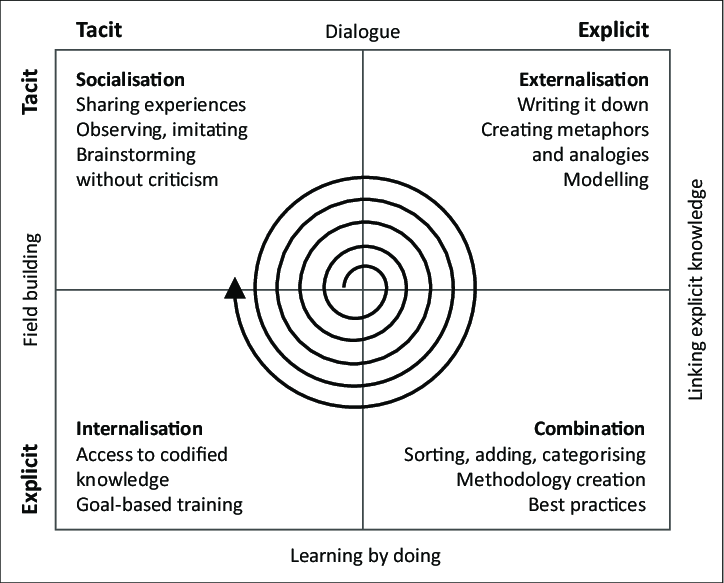
\includegraphics[width=16cm]{images/tacit.png}
    \caption{
        Two dimensional grid showing how the learning processes jump from tacit to 
        explicit learning.
    }
    \label{fig:tacit}
\end{figure}


This type of knowledge is unintuitive and hard to communicate, but it represents a 
very big part of human knowledge, in many cases, knowledge that is vital to the 
communication, interaction and realization of many tasks, on any degree of complexity,
school or professional. The separation of implicit and tacit knowledge is not always
obvious \cite{troublewithtacitknowledge}, but it is believed that implicit knowledge
is just explicit knowledge that hasn't yet been documented, and most of the tacit 
knowledge falls in this category, meaning it can or is in the process of becoming an
understood topic that can be learned and taught logically and systematically.

The conversion between this types of knowledge is fundamental and some strategies 
have been developed for this ending. They usually follow similar principles as the 
traditional ways tacit knowledge is passed on (observation, imitation, etc.). This
principles observed in musical instrument learning, or bicycle riding can be 
standardized and systematized following some steps:

\begin{itemize}
    \item \textbf{Continuous Learning:} similar to the above mentioned methods, 
        a continuous learning strategy has proven essential when adapting the transfer
        of tacit knowledge as explicit.
    \item \textbf{Current Knowledge Auditing:}
        the act of verbalizing the existing knowledge by auditing and identifying 
        knowledge gaps is one of the most important steps in understanding and 
        codifying it.
    \item \textbf{Build Intentional Learning:}
        many times this type of knowledge is transmitted while the authors are 
        unaware. Building attention and intention is imperative to its transition to
        an explicit category.
    \item \textbf{Storytelling Injection:}
        since tacit knowledge is best understood through personal experience, 
        describing it by telling stories as opposed to logical explanations 
        is much more effective when codified.
\end{itemize}



\section{Micro-Learning}
\label{section:micro}

The concept of Micro-Learning is not unique to technology-based learning practices,
even though it is generally used in correlation with the latter. The term is fairly
new compared to its counter part, micro teaching \cite{microlearningdimensions}. 
In the sixties in the University of Stanford, USA, new methods of teaching started 
being developed with much criticism to the then state-of-the-art as exposed by 
Dwight \& Ryan 1969 \cite{dwight_ryan_1969}. Many Professors of this institution started
to follow a much simpler and shorter cyclical teaching model that iterated over
the following steps:

\begin{itemize}
    \item teach
    \item critique
    \item re-teach
    \item critique
\end{itemize}

This approach to repetitively convey information, reviewing and analyzing it proved
very efficient and the idea of dividing content into micro lessons, micro periods and
laboratory phases has been advanced during the last decades to what is known today
as Micro-Learning. 
Many forms and practices are used in Micro-Learning, according to 
\cite{webservicearchitectureforsocialmicrolearning} the main 
principles that define the concept is content that:

\begin{enumerate}
    \item is self-contained, self-explanatory and can be presented without further context,
    \item comprises a single learning activity that can be performed within seconds, and
    \item provides immediate performance feedback.
\end{enumerate}


Examples of micro learning activities would be reading a paragraph of text, 
listening to an informational podcast, watching a short video clip, viewing a 
flashcard, memorizing a word, vocabulary, definition or formula, sorting a set
of items by chronological order, selecting an answer to a question, answering 
questions in quizzes, playful learning with micro-games, composing a short poem,
writing or drawing a reflection on just-viewed content, rating confidence in an 
answer to a question, etc.


\subsection{Micro-Content}

Inseparable from the concept of Micro-Learning is the one of Micro-Content also referred to as
\textit{content nuggets}. There are 
multiple dimensions to this, but generally small segments and fragments of organized
information can be used to describe Micro-Content.
The adjective micro is used when comparing content in three levels, micro, meso and
macro, the latter being the broader and more generalized and first the smallest and 
more compact as the name implies. In the context of language learning, alphabet and
phonetics would be best taught in micro segments, while conversation skills and 
a broader linguistic comprehension would be considered macro content.
The idea of separating learning content into this three layers can occur in different
dimensions as explained by Hug \cite{microlearningdimensions}:

\begin{itemize}
    \item \textbf{Time:} 
        Ideally, Micro-Content should be fast to deliver, performed with relatively
        short effort with no operating expense.
    \item \textbf{Content:} The content should hold small or very small learning units
        with narrow topics and cover simple issues.
    \item \textbf{Curriculum:} 
        It should only wrap a small subset of the curricular setting, parts of modules
        or small elements of informal learning.
    \item \textbf{Form:} 
        The form of this segments should be divided in fragments or 
        \textit{knowledge nuggets} that isolate skill elements.
    \item \textbf{Process:} The process should be
        separate, concomitant or actual, situated or integrated in activities, such
        that they engage in attention management with complete awareness for a small
        period of time, since they should be encompassed in iterative methods.
    \item \textbf{Mediality:} 
        Preferably this content should be delivered in a direct and fast means of
        transportation, either in face-to-face interaction, mono-media, where the
        information objects or learning objects carry high symbolic value.
    \item \textbf{Learning type:} 
        The kind of learning practices should be repetitive, activist, 
        reflective, pragmatist, 
        conceptionalist, 
        constructivist, connectivist, behaviourist. Learning by example with tasks
        or exercises that are goal oriented with real problem-solving content.
\end{itemize}


\subsection{Micro-Learner}

There are different theories about learning, but the micro, mesa and macro view 
would separate the process of learning into three stages or even levels, where a 
student repeats the learning process starting with a superficial approach where 
he gathers knowledge, and iterates every time more analytically. This process 
if also referred in \cite{adler_1970} on his guide on how to read a book, where he
mentions inspectional reading or skimming, analytical reading and syntopical reading.
These steps could be described as following:

\begin{enumerate}
    \item absorb basic knowledge about a topic or subject (Learning I) - Behaviourism
    \item actively acquire knowledge in a self-determined matter (Learning II) 
    - 
    Cognitivism
    \item finally be able to construct knowledge (Learning III) - Constructivism
\end{enumerate}

Typically, micro-learning systems focus on the Learning I phase. 

\subsection{Behaviorism}

Behaviorism is a systematic approach, methodology and theory of psychology which
was developed in the beginning of the twentieth century. Behaviorism treats 
animals and Humans alike and attempts to explain how they function 
purely by observation, thus completely disregarding any internal components such 
as the mind with thinking and emotions. The main goal of Behaviorism is to predict
and control behavior via observation. Opposed to other theories of psychology, the
behaviorists believe their subjects are born as a \textit{tabula rasa} or with a 
clean state and learn by reinforcement or punishment. According to this theory,
humans or animals have responses to stimuli based purely on their conditioning
and surrounding environment. This conditioning is divided mostly into two 
categories, the classic and operand or behavior conditioning, which explains or 
treats their reactions in different ways. The classic conditioning explains the 
response to stimulus by combining the individual's history, motivation while 
the operand controls and manipulates the result by reinforcing it with a 
consequence such as punishment or reward.

Behaviorism tries to link the subjects' responses to the entire surrounding 
environment, without creating any assumptions of the internal organisms. In 
learning, this can be considered as the most basic form of practicing, where 
reinforcement and repetition shape the future behavior. In the context of 
Micro-Learning or Micro-Content this means that the first phase, in which the 
learner gathers samples he neglects all the thinking and emotions from the learning
process and sticks to his instincts.



\subsection{Cognitivism}

The psychology theory of Cognitivism emerged in the late fifties mainly as a 
reaction to both challenge and dispute the then settled Behaviorism.
Cognitivism as a learning philosophy opposes Behaviorism in that instead of 
guiding the learners towards the desired direction, it uses feedback to assist 
learners to create accurate mental connections of the desired learning Schemas.

Cognitivism denies the "black box" approach of behaviorists and seeks to understand
the Human mind during the learning process. It endeavors to recognize the mental 
patterns needed to store new information and generate individual logic.
According to cognitivists, students have existing structures or Schemas, and 
the information absorbed during the learning process gets selected, processed
and organized to fit and enhance these memory patterns. \cite{hursthouse_johnson_1980}
Attention and memory are essential elements of the learning process, for they 
function as connection to the already existing Schemas and help map and contextualize
new information. 

This process of internal codification of mental structures, following the steps
of planning, goal setting and organization strategies \cite{hursthouse_johnson_1980}, are
responsible for knowledge acquisition and conservation. Learning is though a 
process that depends highly on the what the learner already knows and his or her
methods of acquiring new knowledge. Information can be organized in different 
ways according to the already existing structures, and it is the teachers 
job to convey data in a way that facilitates the conversion in to this structures, 
such as by analogies or other hierarchical relationships. Once information is 
stored and implemented in different contexts it is said to be transferred. \cite{schunk_academic_motivation_1991}

Cognitivism justifies and represents a second level of learning which is retained
in long-term memory and used every time the stored information is applied.




\subsection{Constructivism}

Constructivism is an even further interpretation theory of the learning process 
as explained by Behaviorism and Congnitivism. According to Constructivism, learners
build or construct their own knowledge through personal experience. They give meaning
to information and assemble it upon the foundation of previous learned knowledge, 
hence the name Constructivism.

According to this theory, new knowledge gets absorbed influenced solely on the 
existing one. The learner constructs or stacks the knowledge understanding the new 
information and concepts molded by what he has learned previously. This process is
active \cite{adler_1970} as all types of learning processes are, where aided or 
unaided the leaner must constantly interpret and analyze the new information,
relating it to the existing one, only then creating a new layer of understanding 
when enlightened. This process of active engagement is individual, thus the same 
lessons can create very different outcomes, since the learner decides how to construct
new meaning combining the new information with the already available mental models.

Teachers who wish to convey new meaning as Constructivists, tend to use active 
engaging teaching methods, such as experiments or real-world problems to incite
learners to utilize their understanding and layer them with the new information.

According to John Dewey \cite{dewey_1938}, this process is a highly social one. 
Interaction between learners will enhance their construction of meaning, the same
way physical work will be assembled more effectively if collaborating.
John Dewey defends also that even unaided forms of learning, via books or other 
resources require indirect socially interaction in order for the learning process 
to work effectively. This idea is also shared by a major contributor to this theory,
Lev Vygotsky \cite{vygotsky_1978}, who developed the Social Constructivism, where 
he justifies with a community, the process of making meaning, also labeled by
Cognitivists as meaning transfer, can occur more effectively with sharing and 
negotiating.

Learning exists only in the mind and is an iterative process that keeps updating the
mental models to adapt to new information. Learning is the constant construction 
of our own interpretation of reality.


\section{Technology Acceptance Model}
\label{section:tam}


All the above mentioned topics are important concepts about the science of learning
and ideas that should be tackled by the smart speaker application, either by 
trying to achieve the goals set out in \nameref{cha:introduction} or analyze
the results accordingly. This section 
will summarize an important measuring model that can predict a technology's adoption.
This model was changed and shaped into the evaluation model used in my thesis.

Since technology has become an vital part of our lives in a accelerated and 
unpremeditated transition, the creation and expectation its creators have about its
adoption has turned out to be unanticipated. The fast paced adoption of a certain
technology might seem surprising, the same way another will unexpectedly not be 
widely adopted. This unpredictability about a new technology's adoption has inspired
academics to design a measuring system, that could predict and quantify how it 
shall be accepted by a general or particular public.

One of this models, and perhaps the most widely used and influential is the 
technology acceptance model, also referred under the acronym of TAM.
The TAM has been under scrutiny for years, since its first introduction by Davis
\cite{davis_1986}.
The model focuses mainly on the user's behaviour towards technology in general and
the technology in focus in particular. It does so, by trying to quantify both the
perceived usefulness and perceived ease of use. The adjective perceived is not to 
be disregarded, for it mirrors and takes into consideration above all else, the 
behaviour and attitude the user has towards the object in question, and not an
absolute and objective perception of its usefulness and ease of use.

\begin{figure}
    \centering
    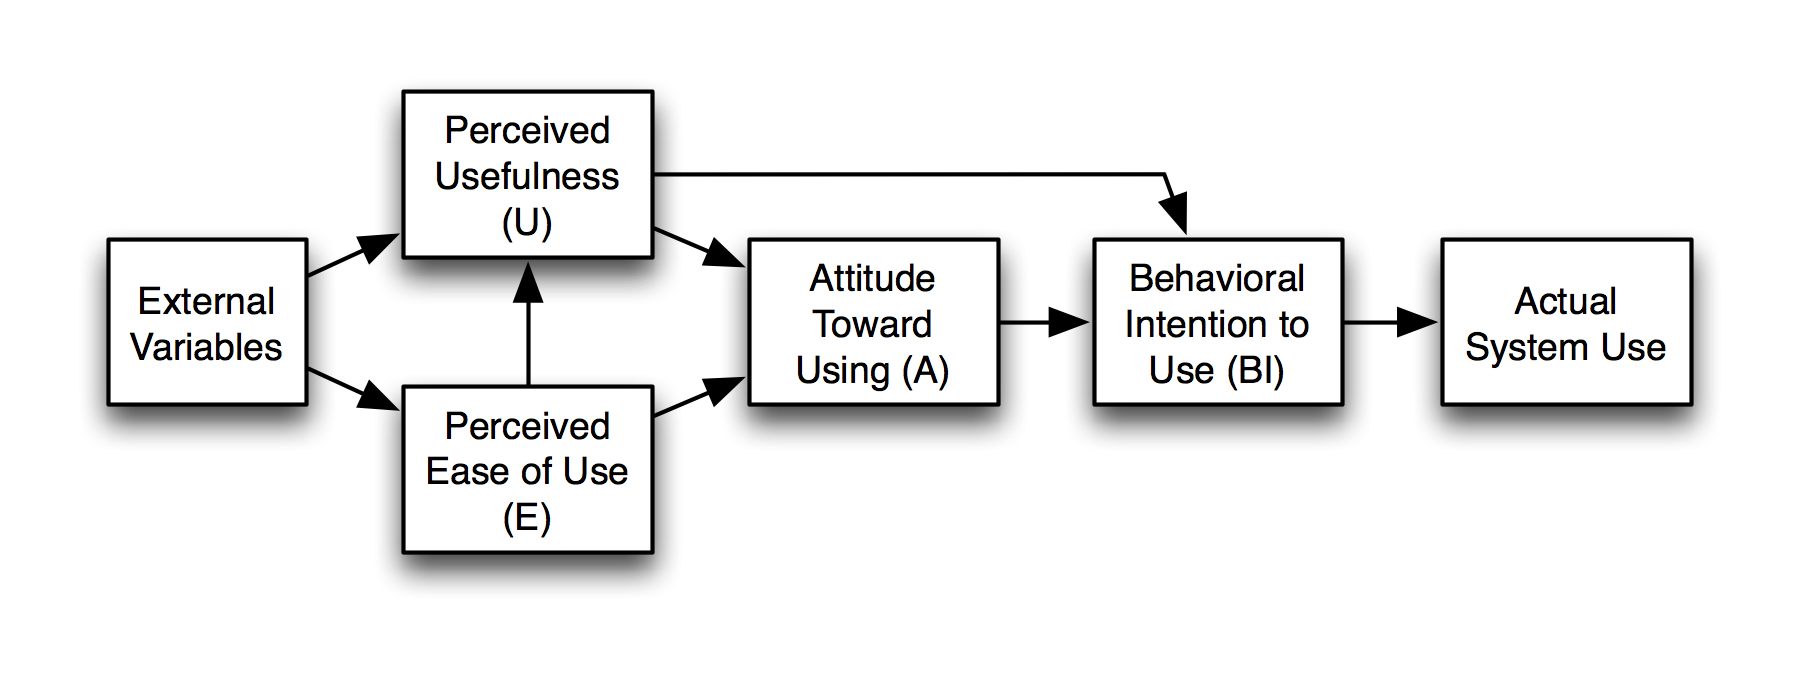
\includegraphics[width=16cm]{images/tam.png}
    \caption{The initial diagram model to describe the technology acceptance model. The two pillars
        of perceived usefulness (PU) and perceived ease of use (PE) have direct influence on the
        attitude (A) and behavioral intention (BI) of the user.
    }
    \label{fig:tam}
\end{figure}

The perceived usefulness attempts to quantify the degree to which a person believes
the use of the technology in question will improve his or hers performance of a 
certain task. How much better will it be to solve a given problem with it, comparing
to without.
The perceived ease of use measurements considers the degree to which a person 
believes the use will be effortless. How much does he/she have to adapt in order 
to operate and employ the technology. Will it be an easy transition.
The entire model revolves around these two fields, which represent different questions
with different directions, but try to evaluate the user's behavior and attitude
towards technology and the one in particular.

The perceived ease of use will also go deeper, by enquiring the user about a 
concept of self-efficacy \cite{lepper_1985}, which stands for the more a user has
contact with the technology, the more control he will feel over the activity it 
covers in general. This self-efficacy also referred to as instrumentality are 
considered to be alongside the attitude, the main factors behind the user's 
motivation, which is essential to the future adopting.

\begin{figure}
    \centering
    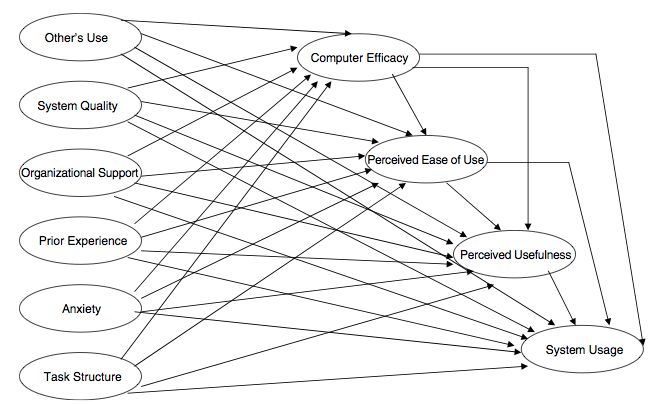
\includegraphics[width=16cm]{images/tam2.png}
    \caption{This diagram represents an expansion to the original TAM as explained in McFarland \& Hamilton 2006 \cite{mcfarland_hamilton_2006}. In this version of the TAM, all external factors influence not only 
    the two pillars PU and PE but also the Computer Efficacy plays a equally important role.
    }
    \label{fig:tam2}
\end{figure}

According to the original TAM, the intention to use a system and perceived usefulness
override the perceived ease of use for the final decision. If the users already has
the intention, he will disregard how difficult it is, if the result proves a positive
a positive outcome.



The TAM is a model that is very general and focuses on psychological aspects that 
vary from experience to experience, from target to target and tends to be adapted
in each study to take into consideration certain aspects. For these reason it has
been consider a parent model to many others, which has inspired other researchers 
to develop an unified model \cite{venkatesh_davis_2000}.

The unified TAM also known as TAM2 takes into consideration other important aspects,
such as:

\begin{itemize}
    \item \textbf{Subjective Norm:}  this stands for the importance the technology in question
        has for the user subjectively. What his opinion of it is, without any objective qualities 
        being taken into account.
    \item \textbf{Voluntariness:} very important is how the user feels it is mandatory to be 
        part and use it. This will affect in many cases the whole approach.
    \item \textbf{Image:} how will the status of the user change in society subsequently to the use
        of adoption plays an important role to certain classes of users. 
    \item \textbf{Job Relevance:} in career fields, this parameter is undeniably vital, to the 
        future users in question.
    \item \textbf{Output Quality:}  this stands for how efficient is the system in question. How will
        the output be in comparison to previously. 
    \item \textbf{Result Demonstrability:} also important is what images are reflected from the results.
        Are the resulting products significantly better, at least the impression of it.
\end{itemize}


\section{Summary}

In this chapter were introduced and explained to a certain extent four learning concepts that are related
to the idea behind this thesis and the base model for its evaluation. 

\nameref{section:cops}, \nameref{section:informal_learning}, \nameref{section:tacit_knowledge} and \nameref{section:micro} are not only
interesting but also ideas that are still being currently explored to understand the depths of human
learning. This still very misunderstood psychological and social processes might define a new future
of efficient learning that is still not recognized, and that can take advantage of the ever increasing
development of new technology.

Smart Speaker is just one proposition in a sea of unexplored hypothesis that can revolutionize 
how humans study and learn in general. The ideas mentioned in this chapter are key to understanding 
how to approach this problem and in creatively innovate the tools available.

\nameref{section:tam} is not the norm but a good base that can interpret and assess how efficient 
the new technologies are and should be an integrative part of any such study. 